\section{Problem 1 Implement Gradient Descent}

\subsection{Initial Guess, Step Size, and Convergence Criteria}
Two functions are used to evaluate the algorithm. $F_1$ is a convex qualdratic bowl.  $F_2$ a superposition of three psedo-multivariate gaussian distributions, which is non-convex.

\begin{figure}[h]
 \centering
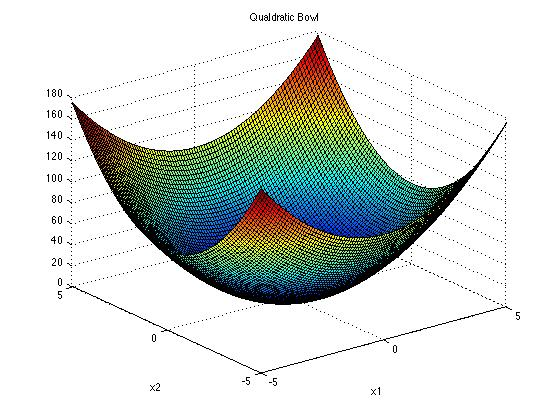
\includegraphics[height=2in]{figures/p1_QualdraticBowl} 
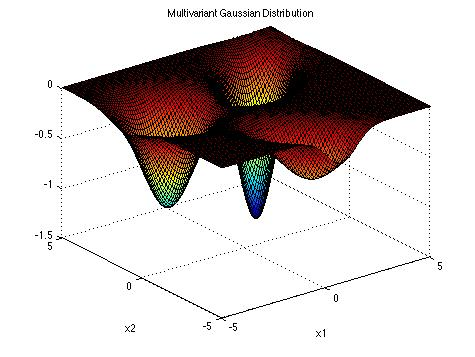
\includegraphics[height=2in]{figures/p1_MultivariantGaussian} 
    \caption{Plots of two functions}
    \label{fig:functions}
\end{figure}

For $F_1$, no matter where the initial guess is, with appropriate step size and convergence criteria, the algorithm will converge at last. Differerent initial guesses result in different iteration numbers. The further the initial guess is from the real optimal, the more iterations it needs to converge. For $F_2$, the intial guess plays a more important role. Since the function is nonconvex and three local minimum exist, the minimum point found by the algorithm could be local minimal but not global minimal. Also, there are 'flat' area exists in this case. The algorithm could converge in two iterations without decsending to the optimums. A very small converge criteria is needed to avoid this. 

\begin{figure}[h]
 \centering
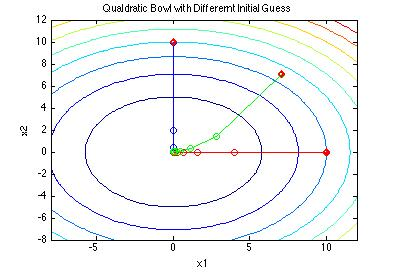
\includegraphics[height=1.8in]{figures/p1_QualdraticBowlWDifferenrtInitial} 
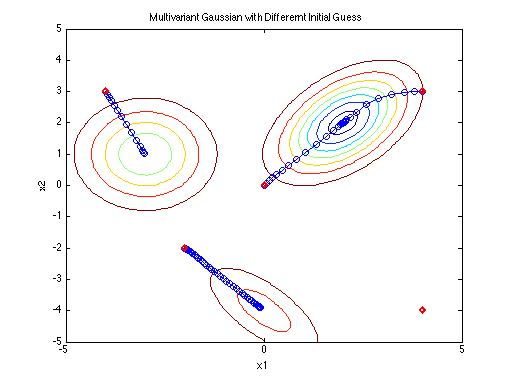
\includegraphics[height=1.8in]{figures/p1_MultivarianGaussianWDifferenrtInitial} 
    \caption{Iteration trajectories from different initial guesses}
    \label{fig:Itr}
\end{figure}

Next, we adjust the stepsize with the inital point and convergence threshold fixed. Only results of $F_1(X)$ are presented however $F_2(X)$ behaves similarly. Table~\ref{tab:ItrStep} shows that, when the stepsize is relatively small, the iteration number decreases as the stepsize increases. However, after the stepsize is large enough, increase the stepsize will help reduce the number iteration no more. Here, when stepsize is 0.2, it takes longer to converge than stepsize is 0.1. If the stepsize further increase, the algorithm may not converge (when stepsize equal or larger than 0.3). From figure~\ref{fig:ItrStep} we can see that, when stepsize is big, the gradient descent trajectory can oscillate around the optimum. Another observation is, a moderate stepsize (in this case 0.1) finds the minimum point of the function with the most accuracy. 

\begin{table}[h]
\centering
\caption{Number of Iteration \& Minimum found v.s. Stepsize} \label{tab:ItrStep} 
\begin{tabular}{ | c | c | c | c | c | c | c | c |  }
\hline 
Stepsize & 0.0001 & 0.0005 & 0.01 & 0.05 & 0.1 & 0.2 & 0.3 \\
\hline 
Iteration num & 878 & 201 & 106 & 22 & 11 & 17 & Not converge \\
\hline
Minimum found $y$ & 0.0081 & 0.0016 & 6.92e-4&9.38e-5 & 3.30e-6 & 3.18e-5\\
\hline
\end{tabular}
\end{table}

\begin{figure}[h]
 \centering
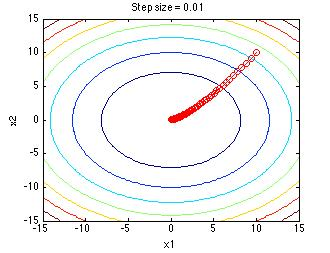
\includegraphics[height=2in]{figures/p1_QualStepSmall} 
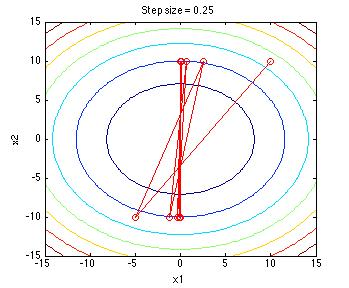
\includegraphics[height=2in]{figures/p1_QualStepBig} 
    \caption{Iteration trajectory with different stepsize (Left) Stepsize=0.01, (Right) Stepsize=0.25}
    \label{fig:ItrStep}
\end{figure}

Finally, we adjust the convergence criteria with the other attributes fixed. Table~\ref{tab:ItrConve} shows that, the smaller the convergence criteria is, the more accurate the found minimum point is, however the longer it takes to converge. Only results of $F_1(X)$ are presented and $F_2(X)$ behaves similar.
\begin{table}[h]
\centering
\caption{Number of Iteration \& Minimum found v.s. Convergence criteria} \label{tab:ItrConve} 
\begin{tabular}{ | c | c | c | c | c | c | c |  }
\hline 
Convergence Criteria & 0.00001 & 0.0001 & 0.001 & 0.01 & 0.1 & 1 \\
\hline 
Iteration num & 12 & 11 & 9 & 8 & 7 & 6  \\
\hline
Minimum found $y$ & 5.28e-7 & 3.30e-6 & 1.29e-4 & 8.05e-6 & 5.00e-3 & 3.15e-2\\
\hline
\end{tabular}
\end{table}


\subsection{Analytical Gradient, Numerical Gradient, and $fminunc()$ }

For $F_1(X)$, we compare the analytical and numerical results on $9 \times 9$ points, given both $x_1$  and $x_2$ vary on 9 values: $[-1000 -100 -10 -1\  0\  1\  10\  100\   1000]$. The difference between the two gradient are controlled under the order of $10^{-8}$ with $\delta = 0.1$. Smaller $\delta$ will give even smaller difference between the analytical and numerical results. $F_2(X)$ requires smaller $\delta$ to make sure the numerical gradient doesn't differ too much from the analytical one. With $\delta = 0.0001$, the difference between the two gradient can again be controlled under the order of $10^{-8}$.

When comparing our algorithm with the matlab $fminunc()$ function, we found our algorithm takes longer to converge. For $F_1(X)$, $fminunc()$ takes around 5 iterations to converge, and the iteration number is not sensitive to the initial guess. For $F_2(X$,  $fminunc()$ is also more efficient and the 'trapped in flat area' phenomena is not observed. However local minimum cannot be avoided.

























